\documentclass[a4paper,twoside]{article}

\usepackage{epsfig}
\usepackage{subfigure}
\usepackage{calc}
\usepackage{amssymb}
\usepackage{amstext}
\usepackage{amsmath}
\usepackage{amsthm}
\usepackage{multicol}
\usepackage{pslatex}
\usepackage{apalike}
\usepackage[draft]{hyperref}
\usepackage{standalone}
\usepackage{longtable}
\usepackage{pbox}
\usepackage[table]{xcolor}
\definecolor{light-gray}{gray}{0.8}
%\rowcolors{1}{magenta}{cyan}
%\rowcolors{1}{}{light-gray}
\let\oldtabular\tabular
\let\endoldtabular\endtabular
\renewenvironment{tabular}{\global\rownum=0\relax\oldtabular}{\endoldtabular}
\usepackage[acronym,toc,nomain]{glossaries}
\makeglossaries
\usepackage{etex}
\usepackage{makecell}
\usepackage{bytefield}
\usepackage{xcolor,colortbl}
\usepackage{a4wide}
\usepackage[inner=1.5in, outer=1.0in, bottom=1in]{geometry}
\usepackage[utf8] {inputenc}
\usepackage[T1] {fontenc}
% \usepackage{amsmath}
\usepackage{amsthm} % is included in mathtools
\newtheorem{theorem}{Theorem}
\usepackage{mathtools}
\usepackage{relsize}
\usepackage{hhline}
\DeclarePairedDelimiter{\ceil}{\lceil}{\rceil}
\DeclarePairedDelimiter{\floor}{\lfloor}{\rfloor}
\usepackage{amsfonts}
\usepackage{verbatim}
\usepackage{todonotes}
\usepackage{calc}
\usepackage{algorithm}
\usepackage{algorithmicx}
\makeatletter
\renewcommand{\ALG@beginalgorithmic}{\scriptsize}
\makeatother
\usepackage{algpseudocode}
\usepackage{multirow}
\usepackage{array}
\usepackage{styles/arydshln}
\usepackage{styles/pgf-umlsd}
\usepackage{pgfgantt}
\algtext*{EndWhile}% Remove "end while" text
\algtext*{EndIf}% Remove "end if" text
\algtext*{EndFor}% Remove "end for" text
\usepackage{caption}
\usepackage{subcaption}
\usepackage{setspace}
\usepackage{pdfpages}
\usepackage{booktabs}
\usepackage{enumitem}
\setitemize{noitemsep}
\usepackage{wrapfig}
\usepackage{pgfplots}
\usepackage{tikz}
\usetikzlibrary{chains}
\usepgflibrary{shapes.geometric}
\usetikzlibrary{shapes}
\usetikzlibrary{calc}
\usetikzlibrary{arrows}
\usetikzlibrary{automata}
\usetikzlibrary{patterns}
\usetikzlibrary{positioning}
\usepackage{styles/tikz-3dplot}
\usepackage{ifthen}
\usepackage{xifthen}
\usepackage{xstring}
\usepackage{pgfopts}
\usepackage{calc}
\usepackage{rotating}
\usepackage{styles/tikz-uml}
\tikzset{
  labelC node/.style={
    at end,align=center,above=-0.08cm,xshift=-6,sloped,
    font=\footnotesize,
    execute at begin node=\setlength{\baselineskip}{0.7em},
    node distance=5cm        
%     append after command={%    
%     \pgfextra
%       \node[draw,near end]{#1};
%       \node[labelB node,middle]{#2}
%       \node[draw,near start]{#3} 
% %      \node[at end, above right]{#2};     
% %      \node[at end, above right]{#3};
%     \endpgfextra
%     }
  },
  labelD node/.style={    
    at start,align=center,sloped,right=-0.08cm,xshift=6,
    rotate=-90,
    font=\footnotesize,
    execute at begin node=\setlength{\baselineskip}{0.7em},
    node distance=5cm        
  }
}
\newcommand{\conceptionalclassbox}[2]{%
\begin{tikzpicture}
\draw (0,0)  node[rectangle,minimum height=0.7cm,draw,minimum width=2.1cm,align=center](satellite){};
\draw (satellite) node[align=center,font=\scriptsize] {#1};
\draw (satellite) node[minimum height=1cm,minimum width=2.1cm,draw,below of=satellite,align=left,font=\scriptsize,node distance =0.85cm](diagram){};
\draw (diagram.north west) node[anchor=north west,align=left,font=\scriptsize] {#2};
\end{tikzpicture}
}
\tikzset{>=stealth',shorten >=1pt,
  object node/.style={
    circle,align=center,
    minimum size=2cm,inner sep=0pt,
    draw
    % font=\sffamily\normalsize\bfseries
  },
  control node/.style={
    circle,dashed,align=center,
    minimum size=2cm,inner sep=0pt,
    draw
    % font=\sffamily\Large\bfseries
  },
  labelA node/.style={
    midway,align=center,above=-0.08cm,sloped,
    font=\footnotesize,
    execute at begin node=\setlength{\baselineskip}{0.7em},
    node distance=5cm
  },
  labelB node/.style={
    midway,align=center,below=-0.08cm,sloped,
    font=\footnotesize,
    execute at begin node=\setlength{\baselineskip}{0.7em},
    node distance=5cm
  },
  labelKrillo node/.style={
    midway,align=center,right=-0.08cm,yshift=2,
    font=\footnotesize,
    execute at begin node=\setlength{\baselineskip}{0.7em},
    node distance=5cm
  },
  labelInvKrillo node/.style={
    midway,align=center,left=-0.08cm,yshift=2,
    font=\footnotesize,
    execute at begin node=\setlength{\baselineskip}{0.7em},
    node distance=5cm
  },
  data node/.style={
    align=center,
    execute at begin node=\setlength{\baselineskip}{1em},
    append after command={%
      \pgfextra
      \draw [-]  (\tikzlastnode.south east) to (\tikzlastnode.south west);
      \draw [-]  (\tikzlastnode.north east) to (\tikzlastnode.north west);
      \endpgfextra
    }
  },
  terminate node/.style={
    align=center,
    execute at begin node=\setlength{\baselineskip}{0.7em}
  },
  task node/.style={
    trapezium,
    trapezium left angle=50,
    trapezium right angle=-50,
    align=center,
    minimum height=1cm, minimum width=4cm, draw,
    append after command={%
    \pgfextra
        \node[draw=none,fill=none, align=center] at (\tikzlastnode.center) {#1};
    \endpgfextra
    }
  },
  harry_potter1 node/.style={
    align=center,minimum height=1.5cm,
    minimum width=0.5cm, rotate=25, anchor = south,
    append after command={%
    \pgfextra
        \node[draw=none,fill=none, align=center] at ([xshift=10, yshift=7]\tikzlastnode.north) (1) {#1};
        \draw  plot [tension=1] coordinates {(\tikzlastnode.north east) ([xshift=5, yshift=-5]\tikzlastnode.center) ([xshift=-5, yshift=5]\tikzlastnode.center) (\tikzlastnode.south west)};
    \endpgfextra
    }
  },
  harry_potter2 node/.style={
    align=center,minimum height=1.5cm,
    minimum width=0.5cm, rotate=25, anchor = south,
    append after command={%
    \pgfextra
        \node[draw=none,fill=none, align=center] at ([xshift=-5, yshift=-10]\tikzlastnode.south) (1) {#1};
        \draw  plot [tension=1] coordinates {(\tikzlastnode.south west) ([xshift=-5, yshift=5]\tikzlastnode.center) ([xshift=5, yshift=-5]\tikzlastnode.center) (\tikzlastnode.north east)};
    \endpgfextra
    }
  },
  queue_v node/.style n args={3}{
    align=center,midway,anchor=center,
    rotate around={#2:(0,0)},
    minimum height = 10, minimum width = 15,
    append after command={%
    \pgfextra
        \draw node[draw=none, fill=white, anchor=south west, rotate=#2, minimum height = 10, minimum width = 15,] at (\tikzlastnode.south west) {};
        \draw node[anchor=north, rotate=90, align=center, font=\footnotesize,
  execute at begin node=\setlength{\baselineskip}{0.9em}] at ([xshift=10]\tikzlastnode.center) {\footnotesize #1};
          \draw[-] plot coordinates {([yshift=#3*4]\tikzlastnode.north west) (\tikzlastnode.south west) (\tikzlastnode.south east) ([yshift=#3*5]\tikzlastnode.north east)};
          \draw[-] plot coordinates {(\tikzlastnode.north east) (\tikzlastnode.north west) (\tikzlastnode.west) (\tikzlastnode.east) (\tikzlastnode.south east)};
    \endpgfextra
    }
  },
  queue_h node/.style n args={3}{
    align=center,midway,anchor=center,
    rotate around={#2:(0,0)},
    minimum height = 15, minimum width = 10,
    append after command={%
    \pgfextra
        \draw node[draw=none, fill=white, anchor=south west, rotate=#2, minimum height = 15, minimum width = 10] at (\tikzlastnode.south west) {};
        \draw node[anchor=south, rotate=0, align=center, font=\footnotesize,execute at begin node=\setlength{\baselineskip}{0.9em}] at ([yshift=8]\tikzlastnode.center) {#1};
          \draw[-] plot coordinates {([xshift=-#3*4]\tikzlastnode.south west) (\tikzlastnode.south east) (\tikzlastnode.north east) ([xshift=-#3*5]\tikzlastnode.north west)};
          \draw[-] plot coordinates {(\tikzlastnode.north west) (\tikzlastnode.south west) (\tikzlastnode.south) (\tikzlastnode.north) (\tikzlastnode.north west)};
    \endpgfextra
    }
  },
  loose_v node/.style n args={3}{
    align=center,midway,anchor=center,
    rotate around={#2:(0,0)},
    minimum height = 10, minimum width = 15,
    append after command={%
    \pgfextra
        \draw node[draw=none, anchor=south west, rotate=#2, minimum height = 10, minimum width = 15,] at (\tikzlastnode.south west) {};
        \draw node[anchor=north, rotate=90, align=center, font=\footnotesize,execute at begin node=\setlength{\baselineskip}{0.9em}] at ([xshift=10]\tikzlastnode.center) {\footnotesize #1};
        \draw[-] plot coordinates {([yshift=#3*4]\tikzlastnode.north west) (\tikzlastnode.south west) (\tikzlastnode.south east) ([yshift=#3*5]\tikzlastnode.north east)};
    \endpgfextra
    }
  },
  loose_h node/.style n args={3}{
    align=center,midway,anchor=center,
    rotate around={#2:(0,0)},
    minimum height = 15, minimum width = 10,
    append after command={%
    \pgfextra
        \draw node[draw=none, anchor=south west, rotate=#2, minimum height = 15, minimum width = 10] at (\tikzlastnode.south west) {};
        \draw node[anchor=south, rotate=0, align=center, font=\footnotesize,execute at begin node=\setlength{\baselineskip}{0.9em}] at ([yshift=8]\tikzlastnode.center) {#1};
          \draw[-] plot coordinates {([xshift=-#3*4]\tikzlastnode.south west) (\tikzlastnode.south east) (\tikzlastnode.north east) ([xshift=-#3*5]\tikzlastnode.north west)};
    \endpgfextra
    }
  },
  reply_h node/.style n args={4}{
    align=center,midway,anchor=center,
    rotate around={#3:(0,0)},
    minimum height = 15, minimum width = 15,
    append after command={%
    \pgfextra
        \draw node[anchor=center, rotate=0, align=center, font=\footnotesize,execute at begin node=\setlength{\baselineskip}{0.9em}] at ([yshift=(#4*16)+#4*16]\tikzlastnode.center) {\footnotesize #1};
        \draw node[anchor=center, rotate=0, align=center, font=\footnotesize,execute at begin node=\setlength{\baselineskip}{0.9em}] at ([yshift=-#4*22]\tikzlastnode.center) {\footnotesize #2};
        \draw[-] plot coordinates {(\tikzlastnode.south east) (\tikzlastnode.south west) (\tikzlastnode.north west) (\tikzlastnode.north east) ([yshift=#4*15]\tikzlastnode.north east) ([yshift=#4*15,xshift=-#4*16]\tikzlastnode.north east)};
    \endpgfextra
    }
  },
  reply_v node/.style n args={4}{
    align=center,midway,anchor=center,
    rotate around={#3:(0,0)},
    minimum height = 15, minimum width = 15,
    append after command={%
    \pgfextra
        \draw node[anchor=west, rotate=0, align=center, font=\footnotesize,execute at begin node=\setlength{\baselineskip}{0.9em}] at ([xshift=(1+#4)*-24+(1-#4)*8]\tikzlastnode.west) {\footnotesize #1};
        \draw node[anchor=east, rotate=0, align=center, font=\footnotesize, execute at begin node=\setlength{\baselineskip}{0.9em}] at ([xshift=(1+#4)*15]\tikzlastnode.east) {\footnotesize #2};
        \draw[-] plot coordinates {(\tikzlastnode.north east) (\tikzlastnode.south east) (\tikzlastnode.south west) (\tikzlastnode.north west) ([xshift=-#4*15]\tikzlastnode.north west) ([xshift=-#4*15,yshift=-#4*16]\tikzlastnode.north west)};
    \endpgfextra
    }
  },
  data node/.style={
    rectangle,align=center,
    minimum width=2cm,minimum height=1.cm,
    inner sep=0pt,
    draw
   },
   start node/.style={
     circle,fill=black,align=center,
     minimum size=0.75cm,inner sep=0pt,draw
  },
  end node/.style={
     circle, align=center, minimum size=0.75cm, draw,
     append after command = {
     \pgfextra
        \draw node[circle, align=center, minimum size = 0.5cm, fill=black] at (\tikzlastnode.center) {};
     \endpgfextra
     }
  },
  single_queue_v node/.style n args={3}{
    align=center,midway,anchor=center,
    rotate around={#2:(0,0)},
    minimum height = 10, minimum width = 15,
    append after command={%
    \pgfextra
        \draw node[draw=none, fill=white, anchor=south west, rotate=#2, minimum height = 4, minimum width = 15,] at (\tikzlastnode.south west) {};
        \draw node[anchor=north, rotate=90, align=center, font=\footnotesize,
  execute at begin node=\setlength{\baselineskip}{0.9em}] at ([xshift=10]\tikzlastnode.center) {\footnotesize #1};
          \draw[-] plot coordinates {([yshift=#3*4]\tikzlastnode.north west) (\tikzlastnode.south west) (\tikzlastnode.south east) ([yshift=#3*5]\tikzlastnode.north east)};
          \draw[-] plot coordinates { ([yshift=-4]\tikzlastnode.north west) ([yshift=-4]\tikzlastnode.north east) ([yshift=0]\tikzlastnode.south east)};
    \endpgfextra
    }
  }
}

\usepackage{ellipsis}
\usetikzlibrary{calc}
\usetikzlibrary{decorations.pathreplacing,decorations.markings,shapes.geometric}
\tikzset{naming/.style={align=center,font=\small}}
\tikzset{antenna/.style={insert path={-- coordinate (ant#1) ++(0,0.25) -- +(135:0.25) + (0,0) -- +(45:0.25)}}}
\tikzset{station/.style={naming,draw,shape=dart,shape border rotate=90, minimum width=10mm, minimum height=10mm,outer sep=0pt,inner sep=3pt}}
%\tikzset{mobile/.style={naming,draw,shape=rectangle,minimum width=15mm,minimum height=7.5mm, outer sep=0pt,inner sep=3pt}}
\tikzset{mobile/.style={naming,draw,shape=rectangle,minimum width=12mm,minimum height=6mm, outer sep=0pt,inner sep=3pt}}
\tikzset{radiation/.style={{decorate,decoration={expanding waves,angle=90,segment length=4pt}}}}

\newcommand{\MUE}[1]{%
\begin{tikzpicture}[every node/.append style={rectangle,minimum width=0pt}]
\node [mobile,label={[inner ysep=+.3333em]\dots}] (box) {#1};

%\node [mobile] (box) {#1};
%\node at ($(ant1)!0.5!(ant2)$) {\dots};

\draw ([xshift=.25cm] box.south west) circle (4pt)
      ([xshift=-.25cm]box.south east) circle (4pt);

\fill ([xshift=.25cm] box.south west) circle (1pt)
      ([xshift=-.25cm]box.south east) circle (1pt);

\draw ([xshift=.25cm] box.north west) [antenna=1];
\draw ([xshift=-.25cm]box.north east) [antenna=2];
\end{tikzpicture}
}

\newcommand{\UE}[1]{%
\begin{tikzpicture}[every node/.append style={rectangle,minimum width=0pt}]
\node[mobile] (box) {#1};

\draw ([xshift=.25cm] box.south west) circle (4pt)
      ([xshift=-.25cm]box.south east) circle (4pt);

\fill ([xshift=.25cm] box.south west) circle (1pt)
      ([xshift=-.25cm]box.south east) circle (1pt);

\draw (box.north) [antenna=1];
\end{tikzpicture}
}

\newcommand{\MBS}[1]{%
\begin{tikzpicture}
\node[station] (base) {#1};

%\draw[line join=bevel] (base.110) -- (base.70) -- (base.north west) -- (base.north east) -- cycle;
\draw[line join=bevel] (base.100) -- (base.80) -- (base.110) -- (base.70) -- (base.north west) -- (base.north east);
\draw[line join=bevel] (base.100) -- (base.70) (base.110) -- (base.north east);

% original yshift=.8pt
%\draw[line cap=rect] ([xshift=.5cm,yshift=.3pt] base.north) [antenna=1];
%\draw[line cap=rect] ([yshift=.3pt]ant1 |- base.north) -- node[above,shape=rectangle,inner ysep=+.3333em]{\dots} ([xshift=-.5cm,yshift=.3pt]base.north) [antenna=2];
\draw[line cap=rect] ([xshift=-.1768cm,yshift=.6pt]base.north -| base.right tail) [antenna=1];
\draw[line cap=rect] ([yshift=.6pt]ant1 |- base.north) -- node[above,shape=rectangle,inner ysep=+.3333em]{\dots} ([xshift=.1768cm,yshift=.6pt]base.north -| base.left tail) [antenna=2];

%\draw[line cap=rect] ([yshift=.3pt]ant1 |- base.north) -- ([xshift=-.5cm,yshift=.3pt]base.north) [antenna=2];
%\node at ($(ant1)!0.5!(ant2)$) {\dots};
\end{tikzpicture}
}

\newcommand{\BS}[1]{%
\begin{tikzpicture}
\node[station] (base) {#1};

%\draw[line join=bevel] (base.110) -- (base.70) -- (base.north west) -- (base.north east) -- cycle;
\draw[line join=bevel] (base.100) -- (base.80) -- (base.110) -- (base.70) -- (base.north west) -- (base.north east);
\draw[line join=bevel] (base.100) -- (base.70) (base.110) -- (base.north east);

% original yshift=.8pt
\draw[line cap=rect] ([yshift=0pt]base.north) [antenna=1];
\end{tikzpicture}
}

\newcommand{\BSSIMPLE}[1]{%
\begin{tikzpicture}
\node[station] (base) {#1};

%\draw[line join=bevel] (base.110) -- (base.70) -- (base.north west) -- (base.north east) -- cycle;
\draw[line join=bevel] (base.100) -- (base.80) -- (base.110) -- (base.70) -- (base.north west) -- (base.north east);
\draw[line join=bevel] (base.100) -- (base.70) (base.110) -- (base.north east);

\end{tikzpicture}
}
\tikzset{>=stealth',shorten >=1pt,
  computer node/.style={
        rectangle, align=center,
        minimum width=1.4cm,minimum height=1.3cm,draw,
        append after command={
        \pgfextra
        \draw node[draw,minimum width=1.2cm,minimum height=1.1cm] at (\tikzlastnode.center) {};
        \draw node[draw,minimum width=1.5cm,minimum height=0.6cm] at ([yshift=-0.4cm]\tikzlastnode.south) {};
        \draw node[circle, fill=black, minimum size=0.15cm, inner sep=0pt] at ([xshift=0.55cm,yshift=-0.25cm]\tikzlastnode.south) {};
        \endpgfextra
      }
  }
}
\newsavebox{\documentt}
\savebox{\documentt}{
  \begin{tikzpicture}
    \draw (3,4) -- (3,2.75) to[out=-100,in=100] (5,2.75) -- (5,4) -- (3,4);
    % \draw (0,0) -- (1,-0.1666666);
    % \draw (-1.2,0.2) -- (-2.2,0.366666);
    % \draw (-1,0) -- (-2,-0.1666666);
    % \draw (-0.2,0.2) -- (0.8,0.366666);
  \end{tikzpicture}
}


\newsavebox{\cubesatbox}
\savebox{\cubesatbox}{
  \begin{tikzpicture}
    \draw (0,0) rectangle(-1,-1)
    -- (-1.2,-0.8) -- (-1.2,0.2) -- (-1,0) -- (-1.2,0.2)
    -- (-0.2,0.2) -- (0,0);
    \draw (0,0) -- (1,-0.1666666);
    \draw (-1.2,0.2) -- (-2.2,0.366666);
    \draw (-1,0) -- (-2,-0.1666666);
    \draw (-0.2,0.2) -- (0.8,0.366666);
  \end{tikzpicture}
}

\newcommand{\documentTikz}[1]{\scalebox{#1}{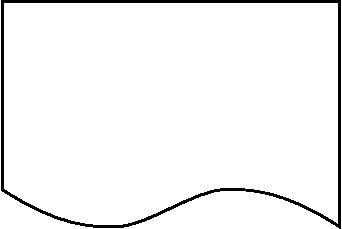
\includegraphics{styles/document.pdf}}}

\usepackage{epstopdf}

\tikzset{
  ciscorouter/.style={align=center,label={center:
      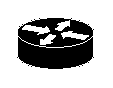
\includegraphics[]{styles/cisco/router.eps}
    },minimum width=0.9cm,minimum height=0.9cm}
}
\tikzset{
  ciscotap/.style={align=center,label={center:
      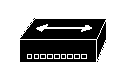
\includegraphics[]{styles/cisco/smallhub.eps}
    },minimum width=0.9cm,minimum height=0.9cm}
}

\usepackage{circuitikz}
\usepackage{multicol}
\newcommand*{\tabbox}[2][t]{\vspace{0pt}\parbox[#1][3.7\baselineskip]{1cm}{\strut#2\strut}}
\usepackage{float}
\usepackage{graphicx}
\usepackage{tabu}
\usepackage{lastpage}
\usepackage{lmodern}
\usepackage[toc,page]{appendix}
\usepackage[titles]{tocloft}
\usepackage{listings}
\usepackage{DejaVuSansMono}
\usepackage{tabularx}
\usepackage{fancyhdr}
\usepackage{cancel}
\setlength{\headheight}{15pt}
\pagestyle{fancyplain}
\usepackage{chngcntr}
\usepackage{footnote}
\makesavenoteenv{tabular}
\makesavenoteenv{table}
\counterwithout{footnote}{chapter}
\usepackage[hang,flushmargin,multiple]{footmisc}
\fancyhf{} % Ingen linje
% Skriv kapitelnavn som lowercase
\renewcommand{\chaptermark}[1]{\markboth{#1}{}}
\lhead[\fancyplain{}{\textit{\thechapter.\ \leftmark}}]{}
\rhead[]{\fancyplain{}{\textit{\leftmark\ \thechapter.}}}
\rfoot[]{\thepage}
\lfoot[\thepage]{}

\definecolor{lightgray}{gray}{0.90}
\newcommand{\colorbitbox}[3]{%
\rlap{\bitbox{#2}{\color{#1}\rule{\width}{\height}}}%
\bitbox{#2}{#3}}

\setcounter{tocdepth}{1}

%\renewcommand{\appendixname}{Bilag}
%\renewcommand{\appendixpagename}{Bilag}
%\renewcommand{\appendixtocname}{Bilag}

\usepackage{caption}
\captionsetup{font=footnotesize,labelfont=bf}
\captionsetup[figure]{labelfont=bf}
\usepackage{titlesec}
\titleformat{\chapter}{\normalfont\LARGE\bfseries}{\thechapter}{1em}{}
\titlespacing*{\chapter}{0pt}{-50pt}{20pt}
%\captionsetup[lstlisting]{labelfont=bf}
\usepackage{MnSymbol}
%\lstset{basicstyle=\scriptsize, tabsize=2, captionpos=b, frame=single}
\lstset{prebreak=\raisebox{0ex}[0ex][0ex]{\ensuremath{\rhookswarrow}}}
\lstset{breaklines=true, breakatwhitespace=true}
\renewcommand{\lstlistingname}{Code}

\lstset{
  language=c,
  basicstyle=\ttfamily\scriptsize,
  identifierstyle=\ttfamily,
  keywordstyle=\ttfamily,
  numbers=left,
  numbersep=5pt,
  xleftmargin=20pt,
  frame=tb,
  framexleftmargin=20pt,
  showstringspaces=false
}

\renewcommand*\thelstnumber{\arabic{lstnumber}:}

\DeclareCaptionFormat{mylst}{\hrule#1#2#3}
\captionsetup[lstlisting]{format=mylst,labelfont=bf,singlelinecheck=off,labelsep=space}


\usepackage{suffix}
\newcommand{\algoref}[1]{Algorithm~\ref{alg:#1}}
\newcommand{\appendixref}[1]{Appendix~-~\emph{\nameref{app:#1}}}
\newcommand{\appendixfigref}[2]{Appendix~\emph{\nameref{app:#1}~-~Figure~\ref{fig:#2}}}
\WithSuffix\newcommand\appendixref*[1]{Appendix~-~\emph{\nameref{app:#1}}}
%\newcommand{\@@appendixref}[1]{Appendix~\emph{\ref{app:#1}}}
\newcommand{\reqref}[1]{Req. \ref{req:#1_long}}
\newcommand{\reqrefnotext}[1]{Req. \ref{req:#1}}
\newcommand{\reqrefshort}[1]{\ref{req:#1_long}}
\newcommand{\reqrefshortnotext}[1]{\ref{req:#1}}
\captionsetup[subfigure]{labelformat=parens}
\newcommand{\subfigref}[1]{(\subref{fig:#1})}
\newcommand{\sectionref}[1]{Section~\emph{\ref{sec:#1}~\nameref{sec:#1}}}
\WithSuffix\newcommand\sectionref*[1]{Section~\emph{\ref{sec:#1}}}
\newcommand{\chapterref}[1]{Chapter~\emph{\ref{sec:#1}~\nameref{sec:#1}}}
\WithSuffix\newcommand\chapterref*[1]{Chapter~\emph{\ref{sec:#1}}}
\newcommand{\figref}[1]{Figure~\ref{fig:#1}}
\newcommand{\listingref}[1]{\lstlistingname~\ref{lst:#1}}
\newcommand{\tableref}[1]{Table~\ref{tab:#1}}
\newcommand{\theoremref}[1]{Theorem~\ref{th:#1}}
\newcommand{\equationref}[1]{Equation~\ref{eq:#1}}


\newcounter{req_counter}
\setcounter{req_counter}{1}

\makeatletter
\newcommand{\reqlabel}[2]{%
  \label{#1}
  \protected@write \@auxout {}{\string \newlabel {#1_long}{{\ref{#1} (#2)}{\thepage}{#2}{#1}{}}}%
  \hypertarget{#1}{#2}
}
\makeatother

\newcommand{\fullfigure}[3]{
  \begin{figure}[ht]
    \centering
    \includegraphics[width=.95\textwidth]{#1}
    \caption{#3}
    \label{fig:#2}
  \end{figure}
}

\newcommand{\fullfigurehere}[3]{
  \begin{figure}[H]
    \centering
    \includegraphics[width=.95\textwidth]{#1}
    \caption{#3}
    \label{fig:#2}
  \end{figure}
}

\newcommand{\fullfigureimport}[3]{
  \begin{figure}[ht]
    \centering
    \input{#1}
    \ifthenelse{\equal{#3}{}}{}{
      \caption{#3}
    }
    \ifthenelse{\equal{#2}{}}{}{
      \label{fig:#2}
    }
  \end{figure}
}

\newcommand{\largefigureimport}[3]{
  \begin{figure}[ht]
    \centering
    \scalebox{0.8}{\input{#1}}
    \ifthenelse{\equal{#3}{}}{}{
      \caption{#3}
    }
    \ifthenelse{\equal{#2}{}}{}{
      \label{fig:#2}
    }
  \end{figure}
}

\newcommand{\mediumfigureimport}[3]{
  \begin{figure}[ht]
    \centering
    \scalebox{0.66}{\input{#1}}
    \ifthenelse{\equal{#3}{}}{}{
      \caption{#3}
    }
    \ifthenelse{\equal{#2}{}}{}{
      \label{fig:#2}
    }
  \end{figure}
}

\newcommand{\smallfigureimport}[3]{
  \begin{figure}[ht]
    \centering
    \scalebox{0.50}{\input{#1}}
    \ifthenelse{\equal{#3}{}}{}{
      \caption{#3}
    }
    \ifthenelse{\equal{#2}{}}{}{
      \label{fig:#2}
    }
  \end{figure}
}

\newcommand{\tinyfigureimport}[3]{
  \begin{figure}[ht]
    \centering
    \scalebox{0.25}{\input{#1}}
    \ifthenelse{\equal{#3}{}}{}{
      \caption{#3}
    }
    \ifthenelse{\equal{#2}{}}{}{
      \label{fig:#2}
    }
  \end{figure}
}

\newcommand{\fullfigureimporthere}[3]{
  \begin{figure}[H]
    \centering
    \input{#1}
    \ifthenelse{\equal{#3}{}}{}{
      \caption{#3}
    }
    \ifthenelse{\equal{#2}{}}{}{
      \label{fig:#2}
    }
  \end{figure}
}

\newcommand{\fullfigureimporttop}[3]{
  \begin{figure}[t]
    \centering
    \input{#1}
    \ifthenelse{\equal{#3}{}}{}{
      \caption{#3}
    }
    \ifthenelse{\equal{#2}{}}{}{
      \label{fig:#2}
    }
  \end{figure}
}

\newcommand{\fullpagefigure}[3]{
  \begin{figure}[hbtp]
    \centering
    \includegraphics{#1}
    \caption{#3}
    \label{fig:#2}
  \end{figure}
}


\newcommand{\fullpagefigureimport}[3]{
  \begin{figure}[hbtp]
    \centering
    \input{#1}
    \caption{#3}
    \label{fig:#2}
  \end{figure}
}

\newcommand{\smallfigure}[3]{
  \begin{figure}[ht]
    \centering
    \includegraphics[width=.55\textwidth,height=.55\textwidth,keepaspectratio]{#1}
    \caption{#3}
    \label{fig:#2}
  \end{figure}
}

\newcommand{\smallerfigure}[3]{
  \begin{figure}[ht]
    \centering
    \includegraphics[width=.50\textwidth,height=.55\textwidth,keepaspectratio]{#1}
    \caption{#3}
    \label{fig:#2}
  \end{figure}
}

\newcommand{\tinyfigure}[3]{
  \begin{figure}[ht]
    \centering
    \includegraphics[width=.25\textwidth,height=.25\textwidth,keepaspectratio]{#1}
    \caption{#3}
    \label{fig:#2}
  \end{figure}
}


\newcommand{\mediumfigure}[3]{
  \begin{figure}[ht]
    \centering
    \includegraphics[width=.65\textwidth,height=.65\textwidth,keepaspectratio]{#1}
    \caption{#3}
    \label{fig:#2}
  \end{figure}
}

\newcommand{\largefigure}[3]{
  \begin{figure}[ht]
    \centering
    \includegraphics[width=.75\textwidth,height=.75\textwidth,keepaspectratio]{#1}
    \caption{#3}
    \label{fig:#2}
  \end{figure}
}

\newcommand{\largerfigure}[3]{
  \begin{figure}[ht]
    \centering
    \includegraphics[width=.85\textwidth,height=.85\textwidth,keepaspectratio]{#1}
    \caption{#3}
    \label{fig:#2}
  \end{figure}
}

\newcommand{\evenlargerfigure}[3]{
  \begin{figure}[ht]
    \centering
    \includegraphics[width=.99\textwidth,height=.95\textwidth,keepaspectratio]{#1}
    \caption{#3}
    \label{fig:#2}
  \end{figure}
}

\newcommand{\largestfigure}[3]{
  \begin{figure}[ht]
    \centering
    \includegraphics[width=1.05\textwidth,height=1.05\textwidth,keepaspectratio]{#1}
    \caption{#3}
    \label{fig:#2}
  \end{figure}
}


% \twofigures{width}{fig1name}{fig1label}{fig1caption}{fig2name}{fig2label}{fig2caption}{overall_label}{overall_caption}
\newcommand{\twofigures}[9]{
  \begin{figure}[H]
	\centering
	\begin{subfigure}[b]{#1\textwidth}
		\centering
		\includegraphics[width=\textwidth]{#2}
		\caption{#4}
        \label{fig:#3}
	\end{subfigure}
    \quad
	\begin{subfigure}[b]{#1\textwidth}
		\centering
		\includegraphics[width=\textwidth]{#5}
		\caption{#7}
        \label{fig:#6}
	\end{subfigure}
	\caption{#9}
    \label{fig:#8}
  \end{figure}
}

% \threefigures{width}{fig1name}{fig1caption}{fig2name}{fig2caption}{fig3name}{fig3caption}{fig4name}{fig4caption}{fig5name}{fig5caption}{overall_label}{overall_caption}
\newcommand{\threefigures}[9]{
  \begin{figure}[H]
	\centering
	\begin{subfigure}[b]{#1\textwidth}
		\centering
		\includegraphics[width=\textwidth]{#2}
		\caption{#3}
        \label{fig:#2}
	\end{subfigure}
    \quad
	\begin{subfigure}[b]{#1\textwidth}
		\centering
		\includegraphics[width=\textwidth]{#4}
		\caption{#5}
        \label{fig:#4}
	\end{subfigure}
    \quad
	\begin{subfigure}[b]{#1\textwidth}
		\centering
		\includegraphics[width=\textwidth]{#6}
		\caption{#7}
        \label{fig:#6}
	\end{subfigure}
	\caption{#9}
    \label{fig:#8}
  \end{figure}
}



% Bibliography
\bibliographystyle{IEEE}

\usepackage[footnote,draft,danish,silent,nomargin]{fixme}
\newcommand{\unit}[1]{~\text{#1}}
\newcommand{\rom}[1]{\uppercase\expandafter{\romannumeral #1}}

\newacronym{cnn}{CNN}{Convolutional Neural Network}
\newacronym{pascalvoc}{PASCAL VOC}{Pattern Analysis, Statistical Modelling and Computational Learning Visual Object Classes}
\newacronym{mscoco}{MS COCO}{Microsoft Common Objects in Context}
\newacronym{ilsvrc}{ILSVRC}{ImageNet Large Scale Visual Recognition Challenge}
\newacronym{svm}{SVM}{Support Vector Machine}
\newacronym{nms}{NMS}{Non-maximum Suppression}
\newacronym{map}{mAP}{Mean Average Precision}
\newacronym{roi}{RoI}{Region of Interest}
\newacronym{rpn}{RPN}{Region Proposal Network}
\newacronym{iou}{IoU}{Intersection-Over-Union}
\newacronym{ssd}{SSD}{Single Shot Detector}
\newacronym{yolo}{YOLO}{You Only Look Once}
\newacronym{fcn}{FCN}{Fully Convolutional Network}
\newacronym{rfcn}{R-FCN}{Region-based Fully Convolutional Network}
\newacronym{ion}{ION}{Inside-Outside Net}
\newacronym{rnn}{RNN}{Recurrent Neural Network}
\newacronym{tdm}{TDM}{Top-down Modulation}
\newacronym{fcis}{FCIS}{Fully Convolutional Instance-aware Segmentation}
\newacronym{ohem}{OHEM}{Online Hard Example Mining}
\newacronym{sgd}{SGD}{Stochastic Gradient Descent}
\newacronym{relu}{ReLU}{Rectified Linear Unit}
\newacronym{flops}{FLOPs}{Floating Point Operations}
\newacronym{ap}{AP}{Average Precision}
\newacronym{caffe}{Caffe}{Convolutional Architecture for Fast Feature Embedding}
\newacronym{iqa}{IQA}{Image Quality Assessment}
\newacronym{nr}{NR}{No-Reference}
\newacronym{live}{LIVE}{Laboratory for Image \& Video Engineering}
\newacronym{lcc}{LCC}{Pearson Linear Correlation Coefficient}
\newacronym{srocc}{SROCC}{Spearman Rank Order Coefficient}
\newacronym{ff}{FF}{Fast Fading}
\newacronym{bpp}{BPP}{Bits per Pixel}
\newacronym{dmos}{DMOS}{Difference Mean Opinion Score}
\newacronym{ar}{AR}{Average Recall}
\newacronym{friqa}{FR-IQA}{Full-Reference Image Quality Assessment}
\newacronym{nriqa}{NR-IQA}{No-Reference Image Quality Assessment}
\usepackage{SCITEPRESS}     % Please add other packages that you may need BEFORE the SCITEPRESS.sty package.

\subfigtopskip=0pt
\subfigcapskip=0pt
\subfigbottomskip=0pt

\begin{document}
% http://www.ijcci.org/Home.aspx
\title{R-FCN Object Detection Ensemble based on Object Resolution and Image Quality}

%\author{\authorname{Christoffer B{\o}gelund Rasmussen and Kamal Nasrollahi}
%\affiliation{Visual Analysis of People (VAP) Laboratory, Aalborg University, Aalborg, Denmark}
%\email{cbra12@student.aau.dk, kn@create.aau.dk}
%}

\keywords{Convolutional Neural Networks, Object Detection, Image Quality Assessment, Ensemble Learning.}

\abstract{Object detection can be difficult due to challenges such as variations in objects both inter- and intra-class. Additionally, variations can also be present between images. Based on this, research was conducted into creating an ensemble of Region-based Fully Convolutional Networks (R-FCN) object detectors. Ensemble strategies explored were firstly data sampling and selection and secondly combination strategies. Data sampling and selection aimed to create different subsets of data with respect to object size and image quality such that expert R-FCN ensemble members could be trained. Two combination strategies were explored for combining the individual member detections into an ensemble result, namely average and a weighted average. R-FCNs were trained and tested on the PASCAL VOC benchmark object detection dataset. Results proved positive with an increase in Average Precision (AP) when ensemble members were combined appropriately.}

\onecolumn \maketitle \normalsize \vfill

\section{\uppercase{Introduction}}
\label{sec:introduction}
Object detection is a fundamental area of computer vision that has had a great amount of research over the past decades. The general goal of object detection is to find a specific object in an image. The specific object is typically from a pre-defined list of categories that are of interest. Object detection generally consists of two larger tasks; localisation and classification. Localisation is typically indicated with a bounding-box indicating where a given object is in the image and classification is determined with an associated confidence to a given class. 

Object detection is a challenging problem due to both large scale issues and minute differences between objects. Firstly, there is the challenge of differentiating objects between classes. Depending on the problem at hand the number of potential classes present can be into the thousands or tens of thousand. On top of this, separate object categories can be both very different in appearance, for example an apple and an aeroplane, but separate categories can also be similar in appearance, such as dogs and wolves. These main challenges of object detection stem from two categories which defined per \cite{zhang} as: robustness-related and computational-complexitity and scalability-related.

Robustness-related refers to the challenges in appearance variations within the both of intra-class and inter-class. These variations can be categorised into two types as per \cite{schroff} as: object and image variations. Object variations consist of appearance differences between object instances with respect to factors such as colour, texture, shape, and size. Image variations are differences not related to the object instances themselves but rather the actual image. This can consist of conditions such as lighting, viewpoint, scale, occlusion, and clutter. Based upon these differences the task of both classifying a given object as a given class but also differentiating the potentially largely varying objects into the same class is challenging.

Current state-of-the-art in object detection is within the realm of deep learning with CNNs. Deep learning methods are of such a scale that given appropriate data have been able to address the two main challenges mentioned earlier. This is exemplified with almost all leading entries in benchmark challenges such as PASCAL VOC \cite{pascalvoc2010}, ImageNet \cite{imagenet}, and MSCOCO \cite{mscoco} consisting of CNN-based approaches. Additionally, recent trends with \gls{cnn}-based object detection methods have been to incorporate ensembles of networks to further enhance performance. 

One of the main goals of an ensemble system is to reduce the variance incorporated in the training process. An example is to train classifiers on different subsets of the data, creating a number of different ensemble members. The assumption is that the classifiers will make different errors on a given data point. However, by combining the classifiers the errors will be mitigated by the increased strength from lower individual variance. The ensemble members created in this work address two of the three main strategies from \cite{ensemblebook} to build an ensemble system. Namely:

\begin{enumerate}
	\item Data sampling and selection: selection of training data for individual classifiers.
	\item Training member classifiers: specific procedure used for generating ensemble members.
	\item Combining ensemble members: combination rule for obtaining ensemble decision.
\end{enumerate}

The robustness-related challenges are addressed by exploring the possibilities of designing expert ensemble members towards both object and image variations in a leading object detection benchmark. This is done by training an ensemble of \gls{rfcn} with ResNet-101 networks. Data sampling strategies are used to create subsets of data with respect to object resolution and various image quality factors. Finally, two separate combination strategies are explored for combining the ensemble members.

\section{\uppercase{Related Work}}
One of the first methods to show that \glspl{cnn} could significantly improve object detection was that of R-CNN \cite{rcnn}. The method obtains the name R-CNN based upon a \gls{cnn} is used on regions of the image. Regions are pre-computed as proposals using a method such as SelectiveSearch \cite{selectivesearch} to give an indication as to where objects may be located. In R-CNN the \gls{cnn} model is used as a feature extractor from which a class-specific linear \gls{svm} can be trained on top of. The AlexNet-based feature extractor is firstly pre-trained on a large dataset designed for classification and then fine-tuned to object detection. Each pre-computed region proposal is run through a forward pass of the model to extract features and then passed to the \gls{svm}.

The R-CNN method was improved the following year with Fast R-CNN \cite{fastrcnn} and aimed to improve speed and accuracy. One of the significant changes is that training end-end rather than in the multi-stage pipeline in R-CNN. A \gls{cnn} is again used as a feature extractor where \gls{roi} pooling is conducted on the final feature map. Afterwards the forward pass continues through two fully-connected layers followed by two sibling output layers replacing the external \gls{svm}. The sibling outputs are a softmax classification layer that produces probabilities for the object classes and another layer for bounding-box regression. In R-CNN, the only deep network used was AlexNet \cite{alexnet}, however, in Fast R-CNN the authors experiment with networks of different size. It was found that the deeper network VGG-16 \cite{vgg16} for computing the convolutional feature map gave a considerable improvement in performance. As the name implies the main improvement is the speed in respect to both training and testing. By computing a convolutional feature map for an entire image rather than per object proposal the number of passes in the network is lowered significantly. While Fast R-CNN provided improvements in both accuracy and speed, the increase in speed is only in relation to the actual object detection and assumes that the region proposals are pre-computed. Therefore, there is still a significant bottleneck per image as a region proposal method can typically take a couple of seconds. 

Faster R-CNN \cite{fasterrcnn} addressed this bottleneck in the third iteration of the R-CNN method. Faster R-CNN showed that region proposals could be computed as part of the network through the use of a \gls{rpn}. The \gls{rpn} shares the convolutional layers and feature map used for computing features with \gls{roi} pooling in Fast R-CNN. As these layers are already computed on the entire image for the classification pipeline, the added time for proposals using the \gls{rpn} is negligible. Apart from the change in how region proposals are computed, there is no difference in comparison to Fast R-CNN. An \gls{rpn} takes the last convolutional feature map as input and returns a number of object proposals.

The winner of the \gls{mscoco} 2015 and \gls{ilsvrc} 2015 detection challenge was with the use of deep residual networks (ResNets) \cite{deepres}. As is well known with \glspl{cnn}, deeper networks are able to capture richer higher-level features. The authors showed that this is also beneficial in the object detection domain. In \cite{deepres} an ensemble of three deep residual networks with 101 layers was trained for object detection and another ensemble of three used for region proposals with the \gls{rpn} while being based on the Faster R-CNN framework. In addition to the ensemble, the winning entry also added box refinement, global context, and multi-scale testing to the Faster R-CNN.

The current leading method on \gls{mscoco} is an extension of the previously explained ResNets \cite{deepres}. This method denoted as G-RMI on the \gls{mscoco} leaderboard \cite{cocolead} is an ensemble of five deep residual networks based upon ResNet \cite{deepres} and Inception ResNet \cite{incepres} feature extractors. No work has been published yet on G-RMI at this time, however, a short explanation of the entry is included in a survey paper from the winning authors \cite{speedacc}. The approach was to train a large number of Faster R-CNN models with varying output stride, variations on the loss function, and different ordering of the training data. Based upon the collection of models, five were greedily chosen based upon performance on a validation set. While performance on the models were important, the models were also chosen such that they were not too similar. 

Recently, a newer approach to region-based methods has been proposed with the use of \glspl{fcn} through the \gls{rfcn} \cite{rfcn}. The overall approach is similar to that used in region-based methods such as \cite{rcnn}, \cite{fastrcnn} and \cite{fasterrcnn}. First compute region proposasls using a region proposal method and second perform classification on these regions. \gls{rfcn} uses the \gls{rpn} from Faster R-CNN \cite{fasterrcnn} for proposal computation. However, \gls{roi} pooling is performed on position sensitive score maps rather than the last feature map. The score maps are split up to represent a relative position in a $k\times k$ grid, with each cell presenting information relative to the spatial position of an object. 

\section{\uppercase{Object Detection with R-FCN}}
One of the current leading object detection methods is the \gls{rfcn} \cite{rfcn}. The authors of \gls{rfcn} were inspired by the recent advances in \gls{fcn} classification networks. \gls{rfcn} uses position-sensitive score maps computed by a bank of convolutional layers. The maps add translation variance into the detection pipeline by computing scores in relation to position information with respect to the relative spatial position of an object. A \gls{roi}-pooling layer is added after the score-maps, however, no convolutional operations are done after this point ensuring translation variance.

The overall approach of the \gls{rfcn} also consists of the popular two-stages of region proposal and region classification. Region proposal is done using the \gls{rpn} from Faster R-CNN followed by the position-sensitive score maps and \gls{roi} pooling for region classification. Similar to Faster R-CNN, convolutional layers are applied on the input image and the \gls{rpn} computes region proposals. After this position-sensitive score maps aid in classification.

\begin{comment}
    \begin{figure}[H]
      \centering
        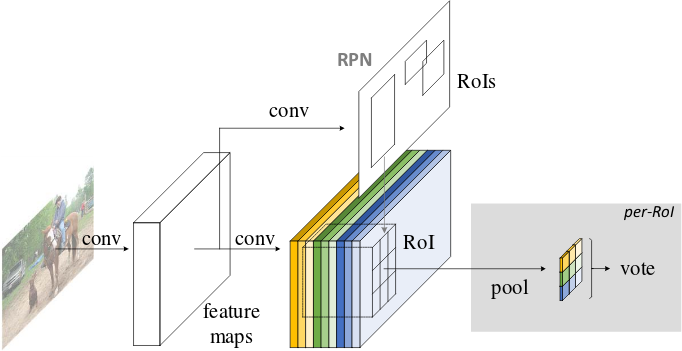
\includegraphics[width=0.8\columnwidth]{Figs/rfcnarchi.png}
          \caption{Architecture of \gls{rfcn}. Region proposals are found using the \gls{rpn} followed by classification based on a bank of position-sensitive score maps \cite{rfcn}.}
        \label{fig:rfcnarch}
\end{figure}
\end{comment}

The added translation variance post finding proposals with the \gls{rpn} is done by producing a bank of $k^2$ score maps for each object category. Therefore, there are a total of $k^2(C + 1)$ maps. The number of $k^2$ maps is due to a $k \times k$ spatial grid representing relative positions. Typically $k = 3$, therefore, nine score maps represent position-sensitive scores for a given object category. For a given \gls{roi} placement the vote for relative position is sampled from their respective map in the bank.

Once the bank of score maps have been computed, position-sensitive \gls{roi}-pooling is found for region classification. Each individual $k \times k$ bin pools from its corresponding location in the relevant score map. For example, the top left bin pools from that position in the top-left score map and so on. The final decision for a given class is determined by a vote where each of the bins are averaged, producing a $(C+1)$-dimensional vector for each \gls{roi}.

\section{\uppercase{Proposed Method}}
An ensemble of \glspl{rfcn} with the ResNet-101 model will be trained towards different robustness-related challenges in the \gls{pascalvoc} dataset. The data used will follow the leading methods for \gls{pascalvoc} 2007 object detection. Training will be done on the 07+12 train sets and testing was conducted on the 07 test set. Evaluation was conducted using the \gls{ap} metric as per the 07 guidelines.

Leading object detection systems take advantage of ensemble methods. Many of them are trained with regards to the variations in internal architecture and not specifically training experts towards solving specific challenges. Therefore, the system in this work will take advantage of the first ensemble strategy from \cite{zhang}, data sampling and selection. The individual \glspl{rfcn} were trained on different subsets of training data with the aim to create expert ensemble members in regards robustness-related challenges, namely object resolution and image quality. 

The third strategy in building an ensemble system, to combine predictions from individual members of the ensemble is also addressed. Bounding-boxes and the confidence of each detection will be combined using an averaging and a weighted averaging method are tested on a number of different combinations of ensemble members.

\subsection{Training Ensemble Members}\label{sec:trainens}
The training of the R-FCN members will be done using \gls{caffe} \cite{caffe}. This was chosen due to the research being available from the authors of R-FCN through training code and pre-trained \gls{caffe} models. As there is the requirement to combine detections between ensemble members, the detections must be found based upon the same input to each model. This is ensured by using pre-computed region proposals found using an \gls{rpn}. In a standard R-FCN the \gls{rpn} is an internal part of the network and is trained end-to-end. However, as these proposals must be constant between all ensemble members this method is not appropriate. Instead the networks are trained using a method inspired by the 4-step alternating training method presented by the Faster R-CNN authors \cite{fasterrcnn}. The process can be seen in \figref{4steptrain}.

 \begin{figure}[!h]
  \centering
    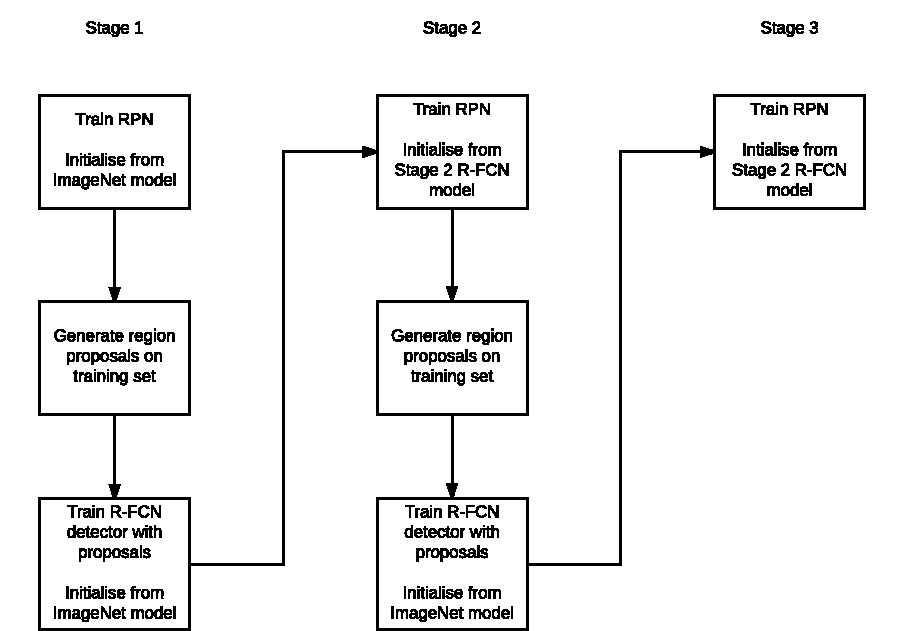
\includegraphics[width=1.0\columnwidth]{Figs/4step-crop.pdf}
      \caption{Flow chart showing the alternating training method.}
    \label{fig:4steptrain}
\end{figure}

In this approach the overall network in trained in multiple steps. First, an \gls{rpn} is trained to determine region proposals, the \gls{rpn} is initialised from a pre-trained ImageNet model and fine-tuned to the proposal task. Next a \gls{rfcn} is trained based upon the proposals found in the previous step. This network is also initialised with a pre-trained ImageNet model. In step three, another \gls{rpn} is trained but initialised using the \gls{rfcn} from step two. In this step the convolutional layers that are shared between the \gls{rfcn} and \gls{rpn} are fixed and only the layers unique to the \gls{rpn} are updated. By training a model with this approach a testing image is able to run through the same steps as a \gls{rfcn} trained end-to-end, however, as the networks are split into different models it is also possible to use the stages of the method individually. Creating a solution for finding region proposals with an external \gls{rpn} and having a number of \glspl{rfcn} that can take the proposals as inputs. 

An additional benefit to training \glspl{rfcn} in this manner is that once a baseline model has been created only one part needs to be re-trained. As the aim is to train various ensemble members to different subsets of data only the \gls{rfcn} in stage 2 is required to be re-purposed. The \gls{rpn} in stage 3 should be kept constant based on the baseline model as it will provide the shared proposals for test images. Therefore, once a systematic approach has been found for splitting data for both train and test based on the data sampling and selection requirements the detection part of the \gls{rfcn} can be trained towards its expert area. The following sections will explain how the subsets of data will be selected.

\subsubsection{Object Size Data Sampling}
The area of a region proposal found with a \gls{rpn} gives an indication as to the approximate size of a potential objects. Therefore, the area for all proposals on the training set can be computed from the output of the second step in stage 2 shown in \figref{4steptrain}. Once the area of all proposals are computed an appropriate split of the data can be determined depending on the area distribution. The main requirement in creating the subsets of data is that equal number of ground truth samples should be present in both.

\subsubsection{Image Quality Data Sampling}
There are many choices for computing the quality of an image and a popular area of research for this purpose is \gls{iqa}. These methods aim to determine the subjective quality of an image. There are two forms of \gls{iqa}, \gls{friqa} and \gls{nriqa}. \gls{friqa} approaches require the original, undistorted reference image in order to determine quality. Whereas, \gls{nriqa} do not have this information available \cite{deepiqa}. As the aim is to determine the level of image quality on one of the benchmark datasets, no reference image is present. Therefore, an \gls{nriqa} method is required. Current state-of-the-art within \gls{nriqa} is also deep learning based and works are typically trained on \gls{iqa} datasets. Datasets include \gls{live} dataset \cite{livepaper} \cite{liveweb}, TID2013 \cite{tid2013} and CSIQ \cite{csiq}. The datasets consist of source reference image and have artificially created counterparts with varying levels of distortion. Distortions include, such as in the LIVE dataset, JPEG2000 compression, JPEG compression, additive white Gaussian noise, Gaussian blur and bit errors from a fast fading Rayleigh channel. Models can then be trained to predict subjective quality based on ground truth user determined quality measurement.

Based upon this, an \gls{nriqa} method can be used to determine the level of image quality with respect to a number of different distortions. Then as in object size training the data will be split into appropriate training subsets. 

\subsubsection{\gls{rfcn} Training}
Training of the baseline \gls{rfcn} model shown in \figref{4steptrain} is done using \gls{sgd} optimisation with largely the same parameters across the five different training parts. The parameters are adapted from \cite{rfcn}. All models start with a base learning rate of 0.001 which is dropped by a factor of 0.1 once in the process. This is done after 80,000 iterations for the \gls{rfcn} models and after 60,000 for the \glspl{rpn}. The learning rate is controlled with a momentum of 0.9 and weight decay of 0.0005. The two \gls{rfcn} models are trained for 120,000 iterations, while the three \glspl{rpn} are trained for 80,000.
The only data augmentation used in training is horizontal flipping of images, effectively creating double the amount of training examples. Additionally, \gls{ohem} \cite{ohem} is used in the training process.

\section{Resolution-Aware Ensemble Members}
To determine an appropriate split of data the distribution of the ground truth bounding boxes area from the 07+12 set was analysed. This was done by parsing all of the bounding box coordinates in the set and calculating the area. A histogram of the all of the ground truth areas can be seen in \figref{0712hist}. There is a clear tendency to smaller objects in the training set with a clear skew towards the left of the figure. The data in \figref{0712hist} can be split into two equal subsets if the median area of 19,205.5 is used as indicated by the red line. 

\begin{figure}[H]
  \centering
    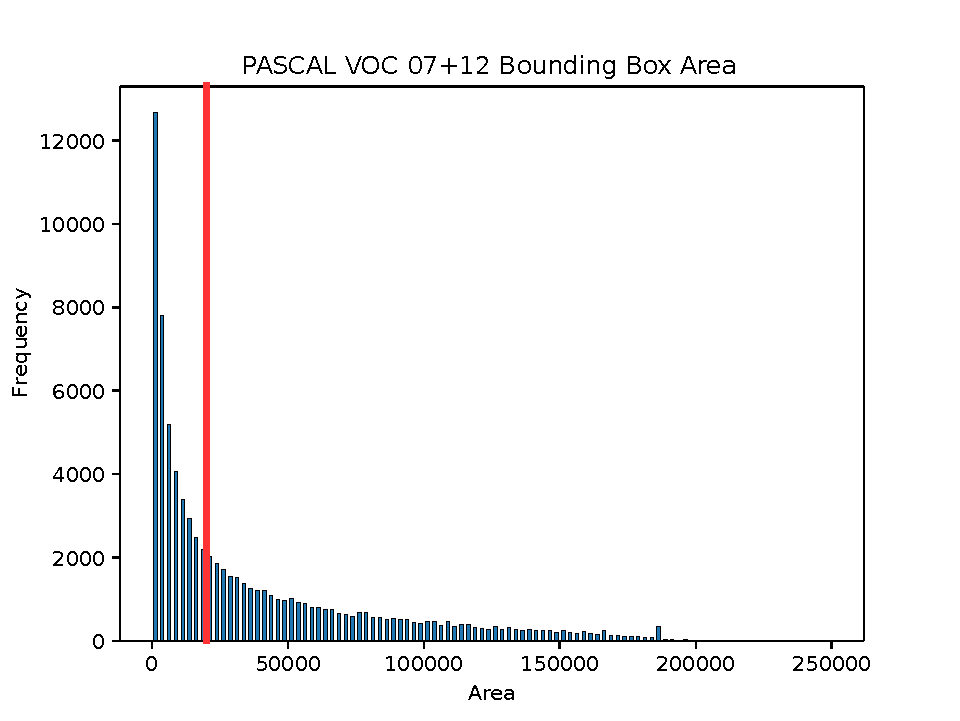
\includegraphics[width=1.0\columnwidth]{Figs/trainvalhistred.pdf}
      \caption{Histogram of the \gls{pascalvoc} 07+12 bounding box area.}
    \label{fig:0712hist}
\end{figure}

However as mentioned, the ensemble \gls{rfcn} members are trained with region proposal inputs of both ground truth positives and negative examples found using a \gls{rpn} as per the multiple step training scheme. A potential shortcoming of using proposals as inputs to training ensemble members is a \gls{rpn} finds many more examples of possible objects than actually are present. Ground truths are determined by setting the proposals with the highest confidence as the ground truth examples and labelling the remaining proposals as the background class. This creates a large difference in the number of samples in comparison to the end-to-end training approach. The total number of training examples is increased from 80,116 ground truth object instances to 9,979,345 region proposals. The median of the almost 10 million proposals is 4,684 pixels, a significantly less than 19,205.5 determined using only ground truth boxes. If the subsets were split by the median of all \gls{rpn} proposals (4,684), the two sets of data would have equal numbers of examples. However, there appears to be a large skew in \gls{rpn} proposals to smaller objects and therefore there significantly more ground truth samples in the subset of data containing larger objects. This can be seen in \tableref{splitrpn}, where despite there being an almost even split in data subsets there are significantly more ground truth annotations in the \gls{rpn}$_{larger}$ subset.

\begin{table}[h]
\centering
\caption{Creating object resolution data subsets. If split by the median area of all region proposals training samples the larger dataset has significantly more ground truth object instance samples.}
\label{tab:splitrpn}
\begin{tabular}{|l|l|l|}
\hline
\textbf{Data} & \textbf{RPN$_{smaller}$} & \textbf{RPN$_{larger}$} \\ \hline
Ground Truth & 19,992    & 60,116     \\ 
Background   & 4,969,369 & 4,929,297  \\ \hline
Total        & 4,989,361 & 4,989,413  \\ \hline
\end{tabular}
\end{table}

Another option is to use the median of 19,205.5 found on only ground truth boxes. The data distribution based on this threshold can be seen in \tableref{splitgt}. In this instance there is significantly more data in the \gls{rpn}$_{larger}$ subset, however, the skew is solely due to the many more background examples. The ground truth annotations are shared equally with 40,058 samples in each.

\begin{table}[h]
\centering
\caption{Creating object resolution data subsets. If split by the median of area from ground truth objects there is an equal number of ground truth instances. However, \gls{rpn}$_{larger}$ has significantly more background samples.}
\label{tab:splitgt}
\begin{tabular}{|l|l|l|}
\hline
\textbf{Data} & \textbf{RPN$_{smaller}$} & \textbf{RPN$_{larger}$} \\ \hline
Ground Truth & 40,058    & 40,058     \\ 
Background   & 3,528,370 & 6,370,859  \\ \hline
Total        & 3,568,428 & 6,410,917  \\ \hline
\end{tabular}
\end{table}

As the overall goal of object detectors is to find objects within the classes, the decision was made to use the threshold of 19,205.5 to create the split in data, despite there being significantly more background examples in one of the datasets.

The \gls{rfcn} ensemble members were trained on the two subsets of \gls{rpn}. To evaluate how well the expert resolution members perform on the respective subsets of data tests were performed on splits of the 07 test data. This data was split by using the same median threshold of 19,205.5 used in creating the training subsets. Firstly, the results for small objects from 07 test can be seen in \tableref{small07res}. Shown are \glspl{rfcn} trained on \gls{rpn}$_{smaller}$, \gls{rpn}$_{larger}$ and a baseline model trained on all 07+12 data. The table shows that the model trained towards smaller object proposals on \gls{rpn}$_{smaller}$ performs best. This trend is similarly true for large objects as seen in \tableref{large07res}. Finally, for all ground truth objects the baseline model is the best performing as seen in \tableref{alldatares}.

\begin{table}[h]
\centering
\caption{Results for \gls{rfcn} models trained on three different subsets of data and tested on only small objects from the 07 test set.}
\label{tab:small07res}
\begin{tabular}{|l|l|}
\hline
\textbf{Train Data} & \textbf{\gls{ap}}      \\ \hline
\gls{rpn}$_{smaller}$      & \textbf{55.00} \\ \hline
\gls{rpn}$_{larger}$      & 20.92 \\ \hline
07+12        & 43.80 \\ \hline
\end{tabular}
\end{table}

\begin{table}[h]
\centering
\caption{Results for \gls{rfcn} models trained on three different subsets of data and tested on only large objects from the 07 test set.}
\label{tab:large07res}
\begin{tabular}{|l|l|}
\hline
\textbf{Train Data} & \textbf{\gls{ap}}      \\ \hline
\gls{rpn}$_{smaller}$      & 21.28 \\ \hline
\gls{rpn}$_{larger}$      & \textbf{81.81} \\ \hline
07+12        & 75.14 \\ \hline
\end{tabular}
\end{table}

\begin{table}[h]
\centering
\caption{Results for \gls{rfcn} models trained on three different subsets of data and tested on all of the 07 test set.}
\label{tab:alldatares}
\begin{tabular}{|l|l|}
\hline
\textbf{Train Data} & \textbf{\gls{ap}}      \\ \hline
\gls{rpn}$_{smaller}$      & 46.74 \\ \hline
\gls{rpn}$_{larger}$      & 62.48 \\ \hline
07+12        & \textbf{79.59} \\ \hline
\end{tabular}
\end{table}

\subsection{Image Quality Ensemble Members}
To evaluate the amount of distortion in the \gls{pascalvoc} dataset a method for \gls{iqa} is needed. A recent state of the art method is that of deep IQA \cite{deepiqa}. Deep IQA is a \gls{cnn}-based \gls{nr} \gls{iqa} method that can be trained to measure the subjective visual quality of an image. Deep IQA consists of 14 convolutional layers, 5 max-pooling layers and 2 fully-connected layers. The convolutional layers are all 3$\times$3 convolution kernels and activated using \gls{relu}. Inputs to each convolutional layer are zero-padded to ensure output size is equal to the input. Max-pooling layers consist of 2 $\times$ 2 sized kernels. The network is trained on mini-batches of 32 $\times$ 32 patches. During inference non-overlapping patches are sampled from the image and image quality scores are predicted for each instance. The patch scores are averaged for the final score for the entire image. 

Deep IQA models were trained using the Chainer framework \cite{chainer} as code and a model trained for all distortions types on the \gls{live} dataset were available from the deep IQA authors. However, to create a more powerful ensemble models were fine-tuned from the model provided towards each of the 5 distortions in the \gls{live}. The training settings are the same as in the deep IQA work apart from the number of epochs in training. As fine-tuning can drastically decrease training time the epochs were decreased from 3,000 to 500.

The models for each distortion type are run through the 07+12 dataset in order to give an indication to the respective distributions. The distributions can been seen in the histograms in \figref{iqdist}.

\begin{figure*}[!h]
\minipage{0.2\textwidth}
  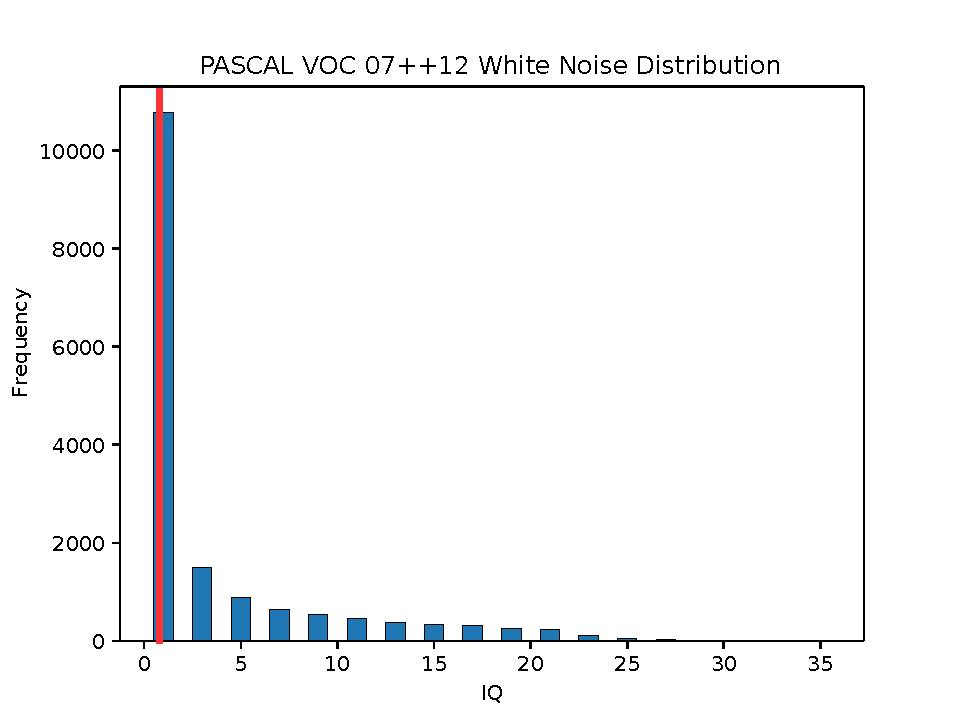
\includegraphics[width=\linewidth]{Figs/WhiteNoisedistred.pdf}
  \caption*{White Noise}\label{fig:dist_wn}
\endminipage\hfill
\minipage{0.2\textwidth}
  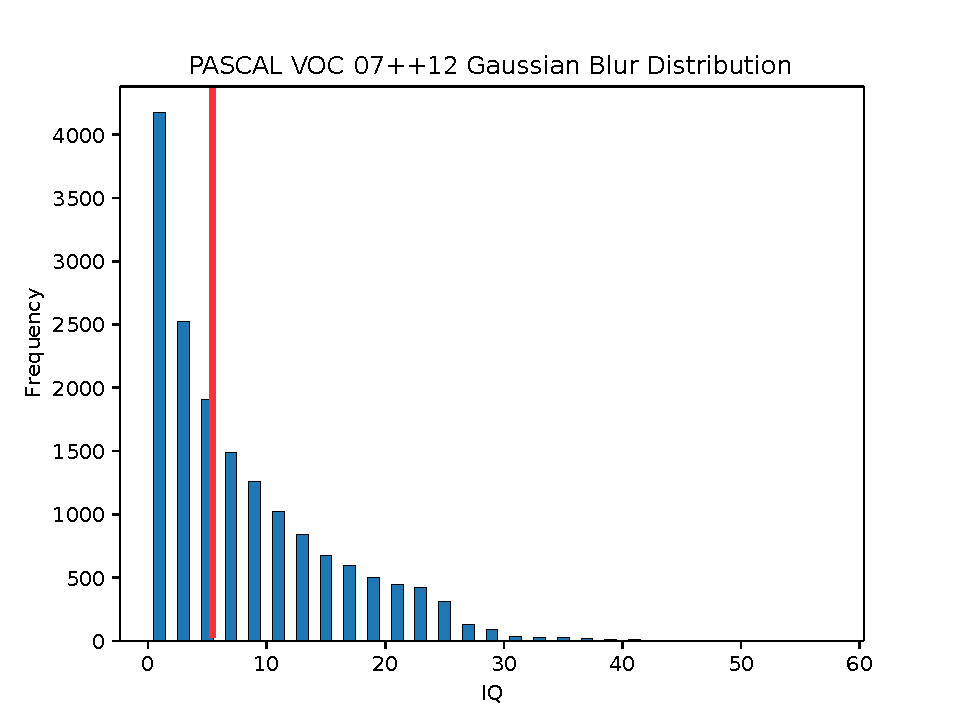
\includegraphics[width=\linewidth]{Figs/GaussianBlurdistred.pdf}
  \caption*{Gaussian Blur}\label{fig:dist_gb}
\endminipage\hfill
\minipage{0.2\textwidth}
  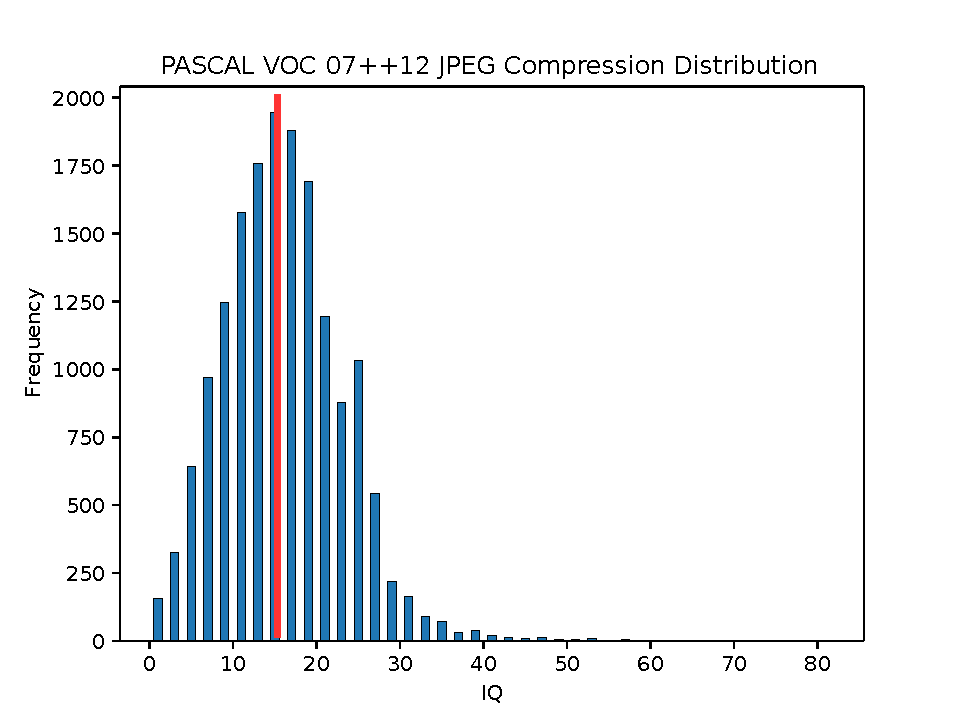
\includegraphics[width=\linewidth]{Figs/JPEGCompressiondistred.pdf}
  \caption*{JPEG}\label{fig:dist_jp}
\endminipage\hfill
\minipage{0.2\textwidth}
  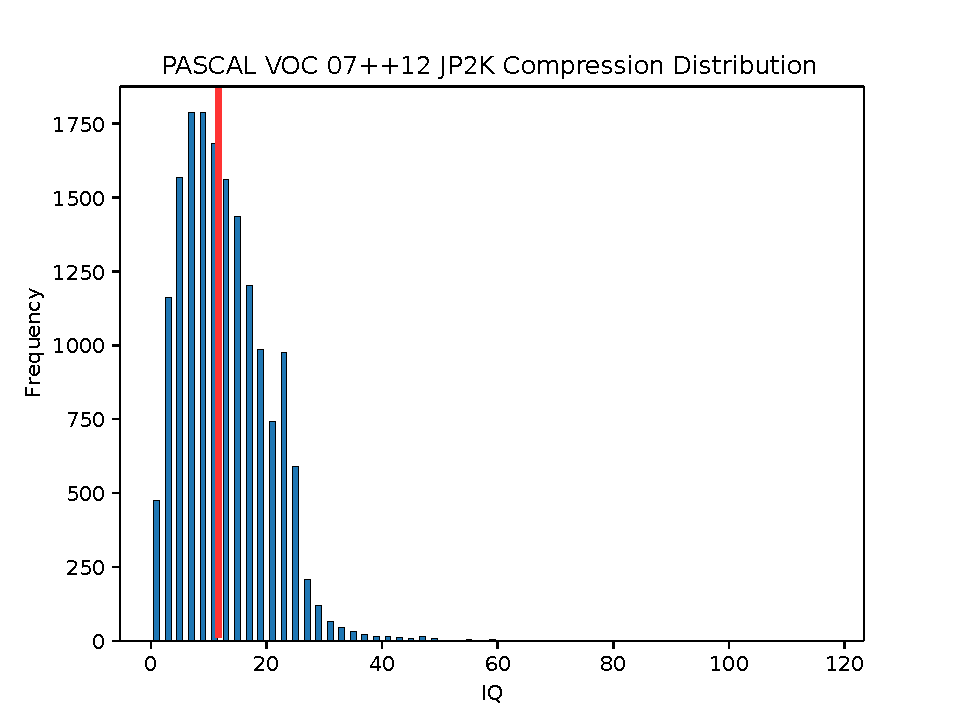
\includegraphics[width=\linewidth]{Figs/JP2KCompressiondistred.pdf}
  \caption*{JP2K}\label{fig:dist_jk}
\endminipage\hfill
\minipage{0.2\textwidth}%
  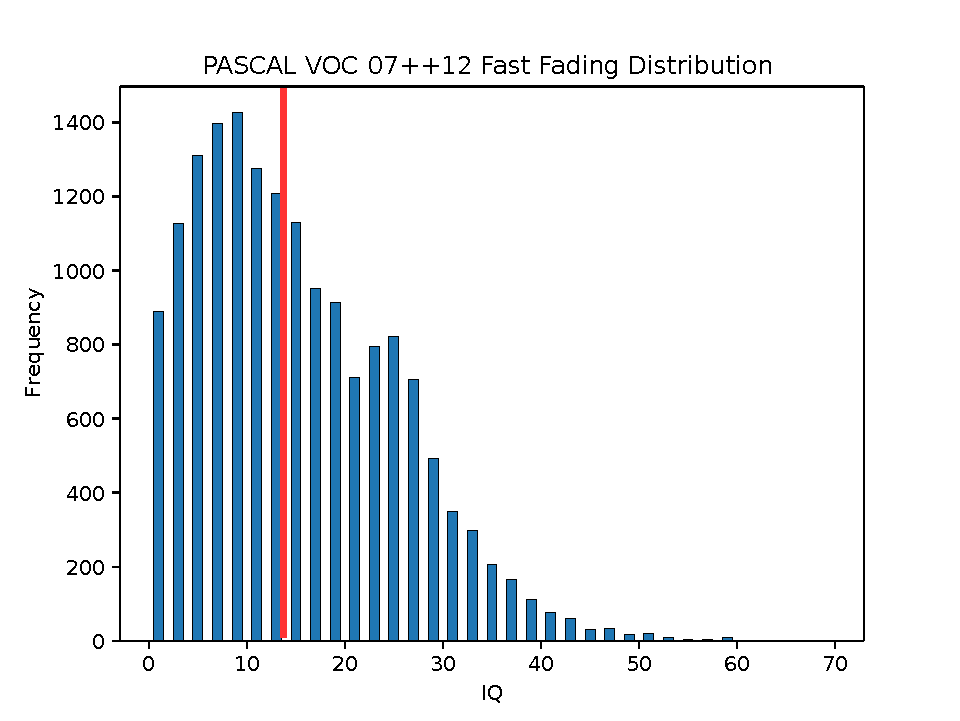
\includegraphics[width=\linewidth]{Figs/FastFadingdistred.pdf}
  \caption*{Fast Fading}\label{fig:dist_ff}
\endminipage
\caption{Histograms representing the distribution of image quality for the five distortions trained from the \gls{live} image quality dataset. The distortions shown are white noise (a), Gaussian blur (b), JPEG compression (c), JP2k compression (d), fast fading (e).}
\label{fig:iqdist}
\end{figure*}

The distribution for white noise and Gaussian blur is skewed towards a higher image quality and also to a lesser extent in fast fading. Whereas the image quality for compression distortions is somewhat of a Gaussian nature. For determining an appropriate manner to split the data the same constraints are made as in that for object sizes, namely that both subsets of data should have an equal number of ground truths to train on. Again using the median for each of the five distributions can satisfy this. The respective medians can be seen in \tableref{iq_splits} and are shown by the red lines in \figref{iqdist}.

\begin{table}[h]
\centering
\caption{Median values used for each distortion type to create even subsets of training data from 07+12.}
\label{tab:iq_splits}
\begin{tabular}{|l|l|}
\hline
\textbf{Distortion Type}   & \textbf{Median} \\ \hline
White Noise       & 0.599  \\ \hline
Gaussian Blur     & 5.607  \\ \hline
JPEG Compression  & 15.660 \\ \hline
JP2K Compression & 11.747 \\ \hline
Fast Fading       & 13.373 \\ \hline
\end{tabular}
\end{table}

It does not appear feasible to create subsets of data for white noise image quality on 07+12. The combination of both the heavy skew and half of the data lying below 0.599 indicates that a minimal amount of white noise distortion is present. Therefore, this distortion is not considered for part of the ensemble. While the Gaussian blur image quality is also skewed it is similar to that of the the object sizes and therefore is deemed appropriate to split based upon its median of 5.607. The remaining distributions are much less skewed and a total of eight R-FCN models will be trained for the high and low levels of image quality for the distortions Gaussian blur, JPEG compression, JP2K compression and fast fading. Therefore, in total there will be ten R-FCN models trained including the two for smaller and larger object sizes.

As in the resolution-aware R-FCN networks individual tests are run to evaluate whether or not the models trained on the above data are candidate experts. The 07 test set is split into lower and upper subsets for each distortion type according to their respective medians. The two respective experts trained on each of their subset and the baseline R-FCN model are evaluated on their respective subsets. Similar results are not found in this instance as in the object resolution experts. For each of the 5 distortions both of the trained experts perform very similarly and are generally 3-4 \gls{ap} lower than the \gls{rfcn} model trained on all of the data. Regardless of this result the following section will present a method to ensemble these members as they may still complement each other. 

\section{Combining the Ensemble Members}
The two strategies, average and weighted average, for combining the ensemble members will be described in this section. The method for inferring each test image will be the same apart from the combination step. For a given object proposal each network will infer a bounding box and associated confidence for all classes. After this the given ensemble combination method determines the final detection where the confidence and the four corners of the bounding box will be averaged. 

\subsection{Average Ensemble}
Each of the five ensemble factors are weighted evenly in the overall ensemble. Within each ensemble factor pair, the detection for one of the pairs will be chosen and the other discarded. This is determined by where the given factor lies for the test image in relation to the training data distribution. For example, if it is measured that an image with a deep IQA model to have JPEG compression below the threshold used to split the data, then the detection found using the model trained on that data will be used. This results in five detections that will be weighted equally to find the final detection by:

\begin{equation}
  E_{j} = \frac{1}{n} \sum_{i=1}^{n} p_{i,j} 
\end{equation}
where $n$ is the number of detections found by the $n$ ensemble factor, $p$ is the detection result to be averaged and $i$ represents one of the ensemble factors. Finally, $j$ is one of the five values found by each detection, namely the four corners of the bounding-box and the associated confidence.


\subsection{Weighted Average Ensemble}
As in the average ensemble, each of the 10 trained networks will be used on all object proposals found using the \gls{rpn}. Between factors, weights are distributed evenly across each of the five different types of factors as in the average ensemble. The weighted average ensemble is determined for each bounding box and the associated confidence by:

\begin{equation}
	E_{j} = \frac{1}{n} \sum_{i=1}^{n} w_ip_{i,j} 
\end{equation}

where $w_i$ is the weight for a given detection.Weights are determined in pairs for each of the 5 ensemble factors, where the total sum of weights is equal to $n$. If each detection were to be weighted equally all $w$ would be equal to 1. As the weights are calculated in pairs each ensemble factor is overall weighted equally as the pair of weights can at most be equal to 2. By using this tactic, detections between ensemble members can be weighted differently but each factor is weighted equally. Weights for a given factor are found according to where the the test image lies for that factors training data distribution. 

If the image factor result $f_i$, for example proposal size, is below the value used to split the data the weights are calculated for the detection found with the given lower network by:

\begin{equation}
	w_{Lower} = 2 - \frac{median_i - f_i}{median_i - minf_i}
\end{equation}

and the weight for the upper network $w_{Upper}$ by:

\begin{equation}
	w_{Upper} = 2 - w_{Lower}
\end{equation}

where $median_i$ is the value used to split the training data and $minf_i$ is the minimum quality for the given factor in the training set.

However, if the quality is above $split$ the $w_{Upper}$ is calculated by:

\begin{equation}
	w_{Upper} = 2 - \frac{maxf_i - f_i}{maxf_i - median_i}
\end{equation}

and lower weight $w_{Lower}$:

\begin{equation}
	w_{Lower} = 2 - w_{Upper}.
\end{equation}

It should also be noted that outliers are not included for the calculation of $minf_i$ and $maxf_i$ by removing the values below the 1\% and above the 99\% percentile. This ensures that the weighing of factors is not too heavily affected by outlier values.

\section{\uppercase{Experimental Results}}
In this section the results for the two aforementioned ensemble combinations strategies will be presented. When appropriate the result for the baseline R-FCN ResNet-101 model trained on all of the 07+12 training data and will be presented and denoted as Baseline. The results presented will be on the 07 \gls{pascalvoc} test set as also shown in earlier preliminary results in this report.

The results for both combination strategies using 10 ensemble members can be seen in \tableref{avgres1}.

\begin{table}[h]
\centering
\caption{Results for the two ensemble combination strategies and for the baseline model on the 07 test set.}
\label{tab:avgres1}
\begin{tabular}{|l|l|}
\hline
\textbf{Method}           & \textbf{\gls{ap}} \\ \hline
Average          & 79.21 \\ \hline
Weighted Average & 79.13 \\ \hline
Baseline         & \textbf{79.59} \\ \hline
\end{tabular}
\end{table}

While neither of the combinations provide an improvement over the baseline method, both have an increase in performance in comparison to their respective image quality expert results. 

To the evaluate the contribution of both the eight quality factor ensemble members and the two resolution members these were combined separately based on the two strategies. By separating the quality and resolution members the performance decreases by roughly 1.0 for both in comparison the the average ensemble result. This appears to indicate that the two complement each other well and have their own expertise for this problem. The weighted average combination strategy does not show as large of a decrease in performance for image quality as the average combination does, however, there is still a drop from 79.13 to 78.44. There is a significant decrease in performance for the two resolution members showing an \gls{ap} of 75.00 on the test set. This seems to show that the addition of weighing individual detections based on proposal size as a poorer approach. There appears to be an indication that image quality members are well suited to adding a weight to detection. Whereas, the resolution members are better suited to simply taking the detection from the appropriate model. The results for this can be seen in \tableref{weandavgres} where both combinations are tested. The two strategies are shown as either Image Quality or Resolution followed by the subscript $_{Avg}$ or $_{WAvg}$ indicating the combination strategies of average or weighted average respectively. 

\begin{table}[h]
\centering
\caption{Results for the the image quality ensemble members and resolution members with both combinations of average and weighted average on the 07 test set.}
\label{tab:weandavgres}
\begin{tabular}{|l|l|}
\hline
\textbf{Ensemble Members}                  & \textbf{\gls{ap}} \\ \hline
Image Quality$_{WAvg}$ / Resolution$_{Avg}$ & \textbf{79.90} \\ \hline
Image Quality$_{Avg}$ / Resolution$_{WAvg}$ & 78.71 \\ \hline
Baseline                          & 79.59 \\ \hline
\end{tabular}
\end{table}

Results in \tableref{weandavgres} show that by using separate strategies where image quality members are weighted and when resolution members are averaged only increases the performance. Additionally, the performance surpasses the baseline model. 

The results so far have only been with different combinations of the expert ensemble members. Another strategy is to include the baseline model trained on all of the 07+12 data. As the baseline model performs well by itself the other ensemble members will act as support It should be noted that as there is no complementary member to the baseline. Therefore, its detections are weighted by 1.0 regardless of ensemble combination strategy. Firstly, the results for the average and weighted average ensemble can be seen in \tableref{ensemble_base}. The inclusion of the baseline model is shown by the subscript $_{base}$. Performance is increased in both cases, the weighted average is increased by 0.22. While the average strategy is increased by 0.65.

\begin{table}[h]
\centering
\caption{Results for the two ensemble combination strategies and for the baseline model on the 07 test set. Shown is both the results with the expert ensemble members only and experts plus the baseline model.}
\label{tab:ensemble_base}
\begin{tabular}{|l|l|}
\hline
\textbf{Method}           & \textbf{\gls{ap}} \\ \hline
Average          & 79.21 \\ \hline
Average$_{base}$          & \textbf{79.86} \\ \hline
Weighted Average & 79.13 \\ \hline
Weighted Average$_{base}$ & 79.35 \\ \hline
Baseline         & 79.59 \\ \hline
\end{tabular}
\end{table}

The addition of the baseline model to the ensemble using different strategies for the two factors can be seen in \tableref{ensemble_comb_base}. This provided the best result of any ensemble combination. Image quality with the weighted average and resolution with average ensemble results in 80.15, an increase of 0.56 in comparison to the baseline \gls{rfcn}.

\begin{table}[h]
\centering
\caption{Results for the the image quality ensemble members and resolution members with both combinations of average and weighted average on the 07 test set.  Shown is both the results with the expert ensemble members only and experts plus the baseline model.}
\label{tab:ensemble_comb_base}
\begin{tabular}{|l|l|}
\hline
\textbf{Ensemble Members}                  & \textbf{\gls{ap}} \\ \hline
Image Quality$_{WAvg}$ / Resolution$_{Avg}$  & 79.90 \\ \hline
Image Quality$_{WAvg}$ / Resolution$_{Avg}$ $_{base}$ & \textbf{80.15} \\ \hline
Image Quality$_{Avg}$ / Resolution$_{WAvg}$ & 78.71 \\ \hline
Image Quality$_{Avg}$ / Resolution$_{WAvg}$ $_{base}$ & 79.10 \\ \hline
Baseline                          & 79.59 \\ \hline
\end{tabular}
\end{table}


The \gls{ap} results for each category for the Image Quality$_{WAvg}$ / Resolution$_{Avgbase}$ ensemble can be seen in \tableref{bestbaseclasses}. The tables show results for the baseline model, the given ensemble method and the difference between the two for a given class. 
 
\begin{table*}[h]
\centering
\caption{Results for the individual classes in the 07 test set. Shown are the results for the baseline model and Image Quality$_{WAvg}$ / Resolution$_{Avgbase}$ . Additionally the difference between the two methods are presented for a given class}
\label{tab:bestbaseclasses}
\resizebox{\textwidth}{!}{%
\begin{tabular}{lllllllllll}
\hline
\multicolumn{1}{|l|}{\textbf{Model}}                                                                           & \multicolumn{1}{l|}{\textbf{aero}}  & \multicolumn{1}{l|}{\textbf{bike}}  & \multicolumn{1}{l|}{\textbf{bird}}  & \multicolumn{1}{l|}{\textbf{boat}}  & \multicolumn{1}{l|}{\textbf{bottle}} & \multicolumn{1}{l|}{\textbf{bus}}   & \multicolumn{1}{l|}{\textbf{car}}   & \multicolumn{1}{l|}{\textbf{cat}}   & \multicolumn{1}{l|}{\textbf{chair}} & \multicolumn{1}{l|}{\textbf{cow}}   \\ \hline
\multicolumn{1}{|l|}{Baseline}                                                                        & \multicolumn{1}{l|}{80.53} & \multicolumn{1}{l|}{84.59} & \multicolumn{1}{l|}{79.89} & \multicolumn{1}{l|}{71.52} & \multicolumn{1}{l|}{67.54}  & \multicolumn{1}{l|}{87.22} & \multicolumn{1}{l|}{\textbf{87.59}} & \multicolumn{1}{l|}{87.98} & \multicolumn{1}{l|}{65.15} & \multicolumn{1}{l|}{\textbf{87.11}} \\ \hline
\multicolumn{1}{|l|}{\begin{tabular}[c]{@{}l@{}}Image Quality$_{WAvg}$ /\\ Resolution$_{Avgbase}$\end{tabular}} & \multicolumn{1}{l|}{\textbf{81.41}} & \multicolumn{1}{l|}{\textbf{85.79}} & \multicolumn{1}{l|}{\textbf{81.09}} & \multicolumn{1}{l|}{\textbf{72.87}} & \multicolumn{1}{l|}{\textbf{69.09}}  & \multicolumn{1}{l|}{\textbf{88.00}} & \multicolumn{1}{l|}{87.42} & \multicolumn{1}{l|}{\textbf{89.12}} & \multicolumn{1}{l|}{\textbf{66.71}} & \multicolumn{1}{l|}{86.72} \\ \hline
\multicolumn{1}{|l|}{Difference}                                                                     & \multicolumn{1}{l|}{+0.88} & \multicolumn{1}{l|}{+1.20} & \multicolumn{1}{l|}{+1.20} & \multicolumn{1}{l|}{+1.35} & \multicolumn{1}{l|}{+1.55}  & \multicolumn{1}{l|}{+0.78} & \multicolumn{1}{l|}{-0.17} & \multicolumn{1}{l|}{+1.14} & \multicolumn{1}{l|}{+1.56} & \multicolumn{1}{l|}{-0.39} \\ \hline
                                                                                                      &                            &                            &                            &                            &                             &                            &                            &                            &                            &                            \\ \hline
\multicolumn{1}{|l|}{\textbf{Model}}                                                                           & \multicolumn{1}{l|}{\textbf{table}} & \multicolumn{1}{l|}{\textbf{dog}}   & \multicolumn{1}{l|}{\textbf{horse}} & \multicolumn{1}{l|}{\textbf{mbike}} & \multicolumn{1}{l|}{\textbf{person}} & \multicolumn{1}{l|}{\textbf{plant}} & \multicolumn{1}{l|}{\textbf{sheep}} & \multicolumn{1}{l|}{\textbf{sofa}}  & \multicolumn{1}{l|}{\textbf{train}} & \multicolumn{1}{l|}{\textbf{tv}}    \\ \hline
\multicolumn{1}{|l|}{Baseline}                                                                        & \multicolumn{1}{l|}{\textbf{73.66}} & \multicolumn{1}{l|}{88.61} & \multicolumn{1}{l|}{\textbf{87.83}} & \multicolumn{1}{l|}{83.21} & \multicolumn{1}{l|}{79.87}  & \multicolumn{1}{l|}{\textbf{54.60}} & \multicolumn{1}{l|}{\textbf{84.07}} & \multicolumn{1}{l|}{\textbf{80.03}} & \multicolumn{1}{l|}{83.60} & \multicolumn{1}{l|}{77.17} \\ \hline
\multicolumn{1}{|l|}{\begin{tabular}[c]{@{}l@{}}Image Quality$_{WAvg}$ /\\ Resolution$_{Avgbase}$\end{tabular}} & \multicolumn{1}{l|}{72.03} & \multicolumn{1}{l|}{\textbf{88.69}} & \multicolumn{1}{l|}{86.96} & \multicolumn{1}{l|}{\textbf{84.24}} & \multicolumn{1}{l|}{\textbf{80.09}}  & \multicolumn{1}{l|}{53.74} & \multicolumn{1}{l|}{83.28} & \multicolumn{1}{l|}{79.88} & \multicolumn{1}{l|}{\textbf{86.28}} & \multicolumn{1}{l|}{\textbf{79.65}} \\ \hline
\multicolumn{1}{|l|}{Difference}                                                                     & \multicolumn{1}{l|}{-1.63} & \multicolumn{1}{l|}{+0.08} & \multicolumn{1}{l|}{-0.87} & \multicolumn{1}{l|}{+1.03}  & \multicolumn{1}{l|}{+0.22}  & \multicolumn{1}{l|}{-0.86} & \multicolumn{1}{l|}{-0.79} & \multicolumn{1}{l|}{-0.15} & \multicolumn{1}{l|}{+2.68} & \multicolumn{1}{l|}{+2.48} \\ \hline
\end{tabular}
%
}
\end{table*}


Finally, two examples of detections can be seen in \figref{boatres}. For both instances, on the left is the full size image and right a zoomed version of the object and detections. The detections shown are for the ground truth annotation, baseline, Resolution$_{base}$ (Res) and Image Quality$_{WAvg}$ / Resolution$_{Avgbase}$ (IQ / Res). Additionally, shown in parentheses in the legend is the \gls{iou} between the ground truth and detection for the given method. 

\begin{figure*}[!h]
\minipage{0.5\columnwidth}
  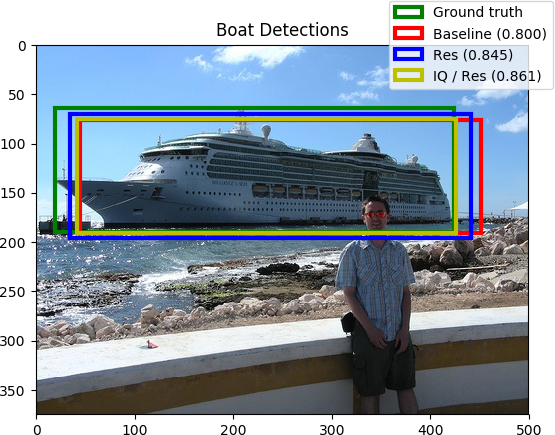
\includegraphics[width=\linewidth]{Figs/000069res.png}
  \caption*{}\label{fig:}
\endminipage\hfill
\minipage{0.5\columnwidth}
  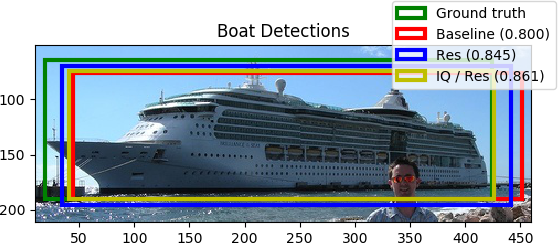
\includegraphics[width=\linewidth]{Figs/000069reszoom.png}
  \caption*{}\label{fig:}
\endminipage\hfill
\minipage{0.5\columnwidth}
  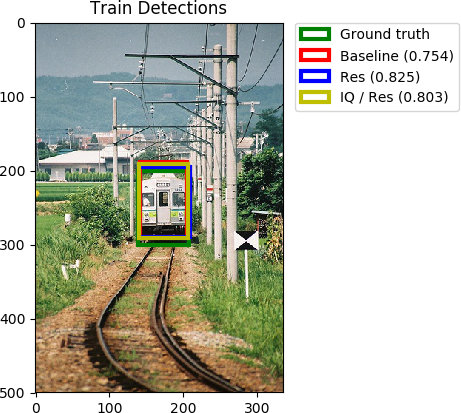
\includegraphics[width=\linewidth]{Figs/000002_res.png}
  \caption*{}\label{fig:}
\endminipage\hfill
\minipage{0.5\columnwidth}
  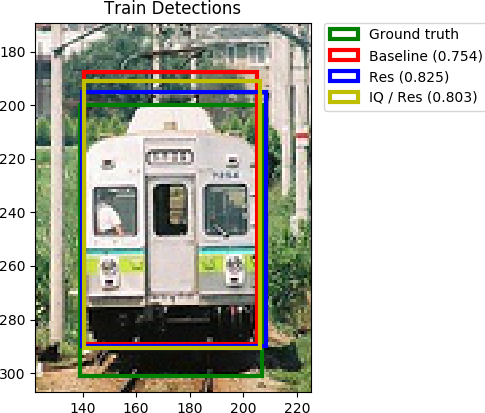
\includegraphics[width=\linewidth]{Figs/000002_reszoom.png}
  \caption*{}\label{fig:}
\endminipage\hfill
\caption{Detections for the boat class from an image in the 07 test set. Shown are the bounding boxes for the ground truth annotation, baseline, Resolution$_{base}$ (Res) and Image Quality$_{WAvg}$ / Resolution$_{Avgbase}$ (IQ / Res). The \gls{iou} between the ground truth and bounding box is shown in parentheses for each method.}
\label{fig:boatres}
\end{figure*}

\begin{comment}
    \begin{figure}[!h]
\minipage{0.2\textwidth}
  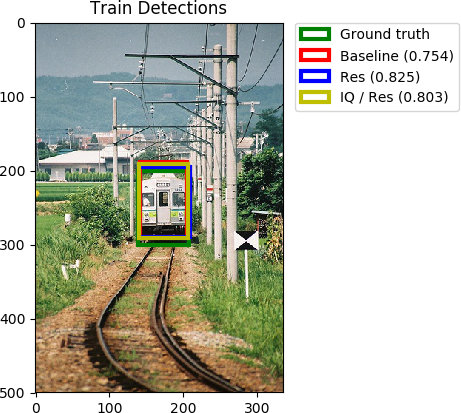
\includegraphics[width=\linewidth]{Figs/000002_res.png}
  \caption*{}\label{fig:}
\endminipage\hfill
\minipage{0.2\textwidth}
  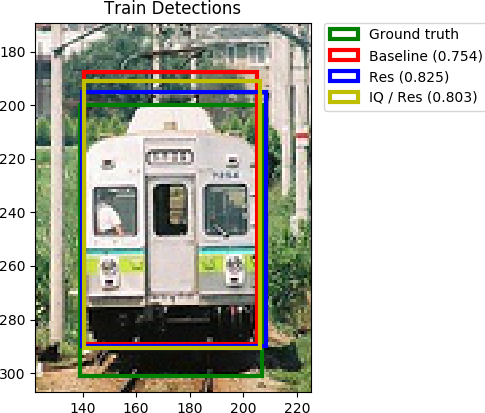
\includegraphics[width=\linewidth]{Figs/000002_reszoom.png}
  \caption*{}\label{fig:}
\endminipage\hfill
\caption{Detections for the train class from an image in the 2007 test set. Shown are the bounding boxes for the ground truth annotation, baseline, Resolution$_{base}$ (Res) and Image Quality$_{WAvg}$ / Resolution$_{Avgbase}$ (IQ / Res). The \gls{iou} between the ground truth and bounding box is shown in parentheses for each method.}
\label{fig:trainres}
\end{figure}

\end{comment}
 
\section{\uppercase{Conclusion and Future Work}}
This work has presented a method for creating an ensemble of \glspl{rfcn} trained towards object resolution and image quality using the \gls{pascalvoc} dataset. If combined appropriately an improvement against the standard \gls{rfcn} method can be obtained. Addressing items such as the skew in factor distributions data may help create better individual members and create a stronger ensemble. 

This work uses \gls{rfcn} as the backbones, however, any object detection method could be used and shows the possibilities of engineering towards specific challenges in object detection.

\bibliographystyle{apalike}
{\small
\bibliography{bibtex}}


\vfill

\end{document}

